\chapter{Sensor effects}

The LSST camera is being constructed at SLAC National Accelerator Laboratory. Its design was motivated by both survey requirements as well as the need to keep with a strict delivery schedule. To this end, a modular design was adopted to enable assembly and testing of individual components in parallel in a test-as-you-build fashion, as well as to allow for the ability to quickly isolate any issues or defects without disturbing the rest of the focal plane.

The camera design is primarily driven by the LSST Camera system and Focal Plane requirements. The fully assembled camera must satisfy these specifications in order to achieve the precision and accuracy needed for scientific analysis. The survey's speed requirements include reaching the 5$\sigma$ limiting magnitudes given in Table \ref{tab:5sigma} in each of the six filter bands. In addition, each patch in the survey footprint will be imaged every three to four nights (in each band?) (LSST system science requirements document, Ivezic). It is therefore essential to minimize the amount of downtime between exposures by enabling a rapid readout of the focal plane. Thus the entire 3.2 gigapixel focal plane will ultimately be read out in two seconds. This is enabled by a CCD pixel architecture consisting of 4k x 4k 10 $\mu m$ square pixels and 16 independent amplifier segments, allowing for a pixel digitization rate of 0.5 MHz.

% Survey depth in each band
% source:  (IVT of LSST Camera Roodman)
\begin{table}
\caption{LSST survey depth requirements.}
\label{tab:5sigma}
\centering
\begin{tabular}{|c|c|c|}
  \hline
  Band & 5$\sigma$ depth per visit & 5$\sigma$ depth over 10 year survey\\
  \hline \hline
  u & 23.9 & 26.1 \\
  \hline
  g & 25.0 & 27.4 \\
  \hline
  r & 24.7 & 27.5 \\
  \hline
  i & 24.0 & 26.8 \\
  \hline
  z & 23.3 & 26.1 \\
  \hline
  y & 22.1 & 24.9 \\
  \hline
\end{tabular}
\end{table}\\


The LSST focal plane consists of 189 CCDs arranged on 21 autonomous cameras called Raft Tower Modules (RTM). An RTM, along with its associated mechanical, thermal and electronic support components, consists of a square matrix of nine CCDs. In addition to the 21 science rafts, there are four additional corner rafts made up of wavefront sensing and guiding arrays used for focusing and telescope guiding.

Although construction of the LSST camera is taking place at SLAC, initial testing of the CCDs and raft assembly begins at Brookhaven National Laboratory (BNL). Once the rafts are completed, they are shipped to SLAC where the results of a similar suite of tests are compared to those obtained at BNL for consistency.

Verification of camera components was performed on a number of testing benches located in the Camera Clean Room at SLAC. I specifically analyzed data from an optical testing bench called Test Stand 8 (TS8), which was used to perform acceptance tests on individual rafts. A subset of the LSST Camera system requirements are shown in Table \ref{tab:cam-req}. TS8 used a 300 Watt Xe arc lamp, a monochromator, a 6-position filter wheel, an OAP feed optic, a 300 millimeter integrating sphere and a 1 meter baffled dark box (LSST Integration & Test subsystem Bond) to produce dark images, flat fields, $^{55}$Fe X-ray sources, and multi-spot images to study noise, linearity, gain, cross-talk, dead pixels, as well as other unexpected instrument signatures. These electro-optical performance tests were run using a software package developed at SLAC called \pkg{eotest}, which is a set of acquisition and analysis scripts used to test the electro-optical performance of the RTMs.  I used the \pkg{eotest} package to study bias and offset corrections, as well as to characterize irregularities in the LSST sensors. Because they were produced by two different vendors, Imaging Technology Laboratory (ITL) and Teledyne e2v (e2v), the CCDs have their own unique signatures due to differences in the manufacturing process. A careful study of sensor effects therefore involved evaluating data from TS8 at the raft, CCD, amplifier and vendor level.

The time I spent at SLAC coincided with the Integration \& Verification Testing phase of the camera construction process, where rafts from BNL were being unpacked from crates and initial verification tests were being performed. 

% Focal plane requirements
% source:  (IVT of LSST Camera Roodman)
\begin{table}
\caption{A subset of LSST Focal Plane requirements.}
\label{tab:cam-req}
\centering
\begin{tabular}{|c|c|c|}
  \hline
  Title & Requirement & Test \\
  \hline \hline
  QE & $>$ 41\%, 78\%, 83\%, 82\%, 75\%, 21\% (u,g,r,i,z,y) & Cam. Calib. wide-beam \\
  \hline
  CCD Diffusion & $\sigma < 5\mu m$ & $^{55}$Fe \\
  \hline
  Read Noise & $< 9e^{-}$ & Bias images \\
  \hline
  Linearity & $<3\%$ & Flat-fields\\
  \hline
\end{tabular}
\end{table}\\ 

\section{Bias and offset studies}
% Need to distinguish between bias and offset

Some of the verification sequences that were taken at TS8, such as flat-fields, darks, and bias images, are used for calibration in order to remove sensor artifacts and thermal noise due to physical processes in the CCD. There are two additional types of pre-processing called bias and offset corrections. Any image can be offset-corrected using data from its overscan region, but removing the bias level requires stacking multiple bias frames. I studied the performance of these pre-processing steps using bias images from TS8. Because they are zero-second exposures taken with the shutter closed, bias frames do not contain any thermally excited or photo-electrons. 

% Offset level is calculated from the image itself, bias is calculated from stacked offset-corrected bias images

% Offset correction
At the end of an exposure, the photo-electrons generated in the bulk silicon go through a capacitor, where their combined charge is registered as a voltage. Since this analog voltage cannot be measured to perfect accuracy, there is some degree of uncertainty when it is translated into digital counts via the analog-to-digital converter. If the signal in a pixel were smaller than the readout noise it could result in that pixel having negative counts. A bias voltage must therefore be applied to the capacitor to ensure that pixels with few or no photo-electrons still register non-negative counts. As a result, every CCD image contains a bulk offset level due to this bias voltage that must be subtracted prior to any scientific analysis. 

The offset level can be thought of as a ``zero-point'', and typically contains around 20,000 counts for LSST sensors. A bias image should look flat overall, with an average count per pixel roughly equal to the offset level. One can measure the offset in an image from the serial overscan region of a single channel in the CCD. The overscan region does not refer to a physical location on the sensor. Rather, this region contains ``virtual" pixels that are the result of continuing the readout process after data from the last physical pixel in the serial register has been recorded. 

I looked at overscan regions of bias images to investigate the performance of various methods of offset correction at the raft, sensor and amplifier level. I then integrated two different offset-correction methods into the \pkg{oetest} software package. At the start of my project, the EOTest package had two ways to calculate the offset level. One was to measure the offset as the mean of all the pixels in the serial overscan region, and the other was to fit a low-order polynomial function to the mean per row in the overscan region. I compared these two methods to three other offset-correction methods: calculating the offset as the mean-per-row in the overscan, as a Gaussian process and cubic spline fits to the mean-per-row in the overscan region. These comparisons can be seen in Fig. [].

% Why do we measure bias from bias images and not other image types? **
% Include image showing CCD architecture and overscan regions
% Include image showing bias results from the Traveler
% How were bias images obtained? What was a typical sequence?
% What type of noise do we expect to see in a bias image?
% I ended up adding mean-per-row and spline fit to mean-per-row **

While the row-by-row correction did the best at characterizing variations in the offset level, it introduced correlated noise of around (read noise / number of columns in overscan) 10/sqrt(50) ~ 1.4 counts per pixel. The cubic spline fit generally did well at fitting the shape of the mean-per-row without adding a significant amount of extra noise. However its performance varied depending on the sensor vendor (it tended to perform better on e2v sensors), as well as on the specific parameters of the spline fit. For example, in some cases, a cubic spline would tend to overfit the data for certain amplifiers, but when the smoothing factor was increased it would come at the cost of losing peaks or dips in the mean-per-row, particularly in the first 50 or so rows. I tried modeling the offset as a Gaussian process to see if it would lead to an improvement, but it actually performed worse at fitting the mean-per-row than the cubic spline fit. 

I modified the \pkg{eotest} package to allow the option to apply a mean-per-row or cubic spline offset correction in addition to the existing mean and polynomial fit functions. After carefully studying these methods and applying them to images from TS8, it was decided that the best way to proceed in terms of the current testing software would be to use the mean-per-row method because, even though it introduces slightly more noise, it is significantly more accurate in the lower rows and would suffice for general performance testing. In the end I made this the default offset-correction method for all electro-optical performance tasks in \pkg{eotest}.

Once the offset level is subtracted and the image is trimmed to remove the overscan region, the next step is to remove the bias level. The bias level is the pixel-to-pixel variations in the read noise in an image. This structure varies from amplifier to amplifier, as well as across a single amplifier in a CCD. To correct for the bias, a `super bias’ is generated for each amplifier by stacking many bias frames that have been offset-corrected and trimmed. This super bias is then used to de-bias other exposures. I added the functionality in \pkg{eotest} to be able to stack a set of images according to a statistic (for example, median-stacking or taking a clipped mean of the stacked images), as well as a method to create a super bias file, which generates a FITS file containing a super bias for each amplifier for a given raft, sensor and run number. 

Next, I did a study of how well the super bias corrected for the bias level. For a given raft, sensor and run number, I first needed to visually confirm each bias image that would be going into the super bias. I will refer to an offset-corrected and de-biased image as a corrected image. I verified all bias images taken during each acquisition mode, which included flat fields, superflats, dark images, quantum efficiency, and an Fe55 source, by plotting serial and parallel projections of each corrected image. This amounted to over-plotting the mean of each row or column in every corrected bias frame against each row or column (see Fig. []). I also plotted the mean and standard deviation over all corrected bias frames as a function of row and column. The mean over all corrected bias images is expected to be zero and the standard deviation is expected to be approximately constant. Bias structure would therefore appear as the mean deviating from zero or sigma varying as a function of row or column. 

Most of the corrected bias images were consistent with no structure, however there was some peculiar behavior in standard deviation as a function of row where I observed random oscillations that varied slowly in time. This is something I did not have a chance to investigate thoroughly, but one potential cause to be investigated is banding, which has been observed in some ITL sensors as a row-wise effect where one can see bands going across the image that vary in bias level. Projecting the bias in this way also revealed an effect called persistence. Several of the corrected bias frames taken during the flat acquisition had mean values as high as 80 counts. A flat-field is an image taken when the sensors are uniformly illuminated. Since flat-field sequences at TS8 involve taking flats at increasingly longer exposure times, they register more light the longer they are exposed. Bias images are taken after every two or three flats in this sequence. Plotting the timestamp of each flat and bias image showed the outlier bias image as the final bias frame taken during this acquisition. Looking at a projection plot of the flat taken just before this bias image showed the flat to have saturated the sensors. It turned out that the excessively high mean value in the outlier bias image was due to charge that had persisted from the previous flat image due to insufficient clearing of the CCD. In this case, more time was needed between parallel pixel transfers during readout. 

% Find an image of banding effect if possible
% Should I go into how flat-fields were taken at TS8?
% Show plot of outlier bias timestamp

Once all bias images that showed anomalous behavior were removed, I created a super bias for all amplifiers on the sensor from 50 bias images. To study the performance of these super biases, I conducted a ``ratio test" using images taken from the superflat acquisition. Superflats were taken in two modes, with low superflats taken to have around 1000 counts, and high superflats having around 50,000 counts. 

The ratio I used to study the super biases was defined as the sum over all corrected low superflats divided by the sum over all corrected high superflats. Because this is essentially a ratio of images, it is immune to any effects like bad pixels or quantum efficiency, which would effectively be divided out. I made a series of two-dimensional histograms of this ratio against the super bias for a number of ITL and e2v rafts. Since the same super bias image is being subtracted from the numerator and the denominator, we would expect the mean of the ratio to be around 1000/50,000 = 0.02 counts, with a sigma of around 0.008. It is also expected that the histogram of the super bias image would have the highest density around zero counts, since the super bias is offset-corrected and should only contain pixel to pixel variations in the noise level. 
% How did I get 0.008?

The results showed a surprising amount of structure in the super biases, particularly in the ITL sensors. For example, there were ``clumps" of points in the super bias that were concentrated in circular lobes at various intervals along the super bias axis. There were also large concentrations of points in the super bias that had values that deviated significantly from zero. On the ratio axis, there were also separate clumps of points, most of which were still centered around 0.02, but some of which had slightly lower or higher mean values. After mapping these questionable pixels onto their physical location on the sensor, most either corresponded to bad columns or to the first few columns of an amplifier. This behavior clearly indicates that something is not correct in the way the super bias is being subtracted, and that there may be pixels that should be masked but are being excluded by the current masking selection process in the \pkg{eotest} code. The e2v sensors were in general more well-behaved, except for a vertical gap around a super bias value of zero, where pixels in the super bias were not being plotted. I verified that these super bias images were indeed masked, so the gaps do not seem to be due to bad masking. But I have yet to investigate whether stacking the super bias using a clipped mean rather than the median would fix this issue. 

Lastly, I studied another issue known as bias trending, which was observed by plotting the mean of the imaging section of all bias images in a run over time. Theoretically, a bias image should only contain the offset level, the bias level and the read noise, the last two of which are sub-dominant. This should make the mean stable around 20,000 counts. However this was not the case and there were significant fluctuations in the mean. My work showed that doing a proper bias and offset correction resolved this instability.

% Show plots

\section{Modeling sky brightness in ImSim}

\subsection{ImSim image simulator}

The success of cosmological surveys depends in large part on the generation of realistic simulations. Synthetic images are used to test software infrastructure such as data processing and analysis pipelines in preparation for the survey, allowing for the study of systematic effects as well as performance testing. Since there is only one observable universe and cosmological parameters cannot be repeatedly measured under exactly identical conditions, we also need simulated data to test different models of the universe once on-sky data is available.

\pkg{ImSim} is a software package developed to fill the need for high-fidelity simulations of Rubin exposures. It is built on top of the GalSim software library to render astrophysical sources as well as the night sky. It also uses telescope and hardware specifications from LSST software libraries describing the telescope PSF and the Rubin focal plane such as CCD geometry and electronics readout. ImSim takes this information as input, as well as descriptions of source positions, spectral energy distributions, magnitudes, cosmological shears and morphologies to produce raw pixel-level data resembling actual data from the Rubin telescope.

% citation: vera c. rubin observatory lsst desc image simulator (chiang et. al)

Each visit on the sky uses a catalog of sources provided by the CatSim package and observing conditions given by the OpSim database. The observing metadata, such as sky brightness and atmospheric seeing, is used by ImSim to calculate the sky background level. 

The initial configuration in \pkg{ImSim} was to calculate the sky level at the center of the focal plane and then use this value for every pixel in the image. This was reasonable as a first-pass, however there was a need to investigate whether this approximation was sufficient enough for capturing variations in the sky level across the focal plane. I studied whether there was a significant enough level of sky variation to warrant a more detailed approach by comparing the existing implementation to a model where the sky level would vary per chip as opposed to maintaining a constant value over every sensor.

To study variations in sky counts per chip I modified the LSST \pkg{skymodel} module, based on the model used by the European Southern Observatory ($https://github.com/lsst/sims_skybrightness$), to give a different sky background for each individual chip. This involved creating a new function that returned the name and pixel coordinates of the centers of each chip. I added a new \pkg{chipName} parameter to the existing sky noise model and converted each pixel coordinate on a chip to its sky coordinates in (ra, dec). Finally, the on-sky chip center positions were passed to the \pkg{skymodel} module to estimate the number of photons incident on the chip for a 30 second exposure (corresponding to two back-to-back 15 second exposures for LSST). Finally, I implemented this new sky model into the \pkg{ImSim} package.

\begin{figure}
\centering
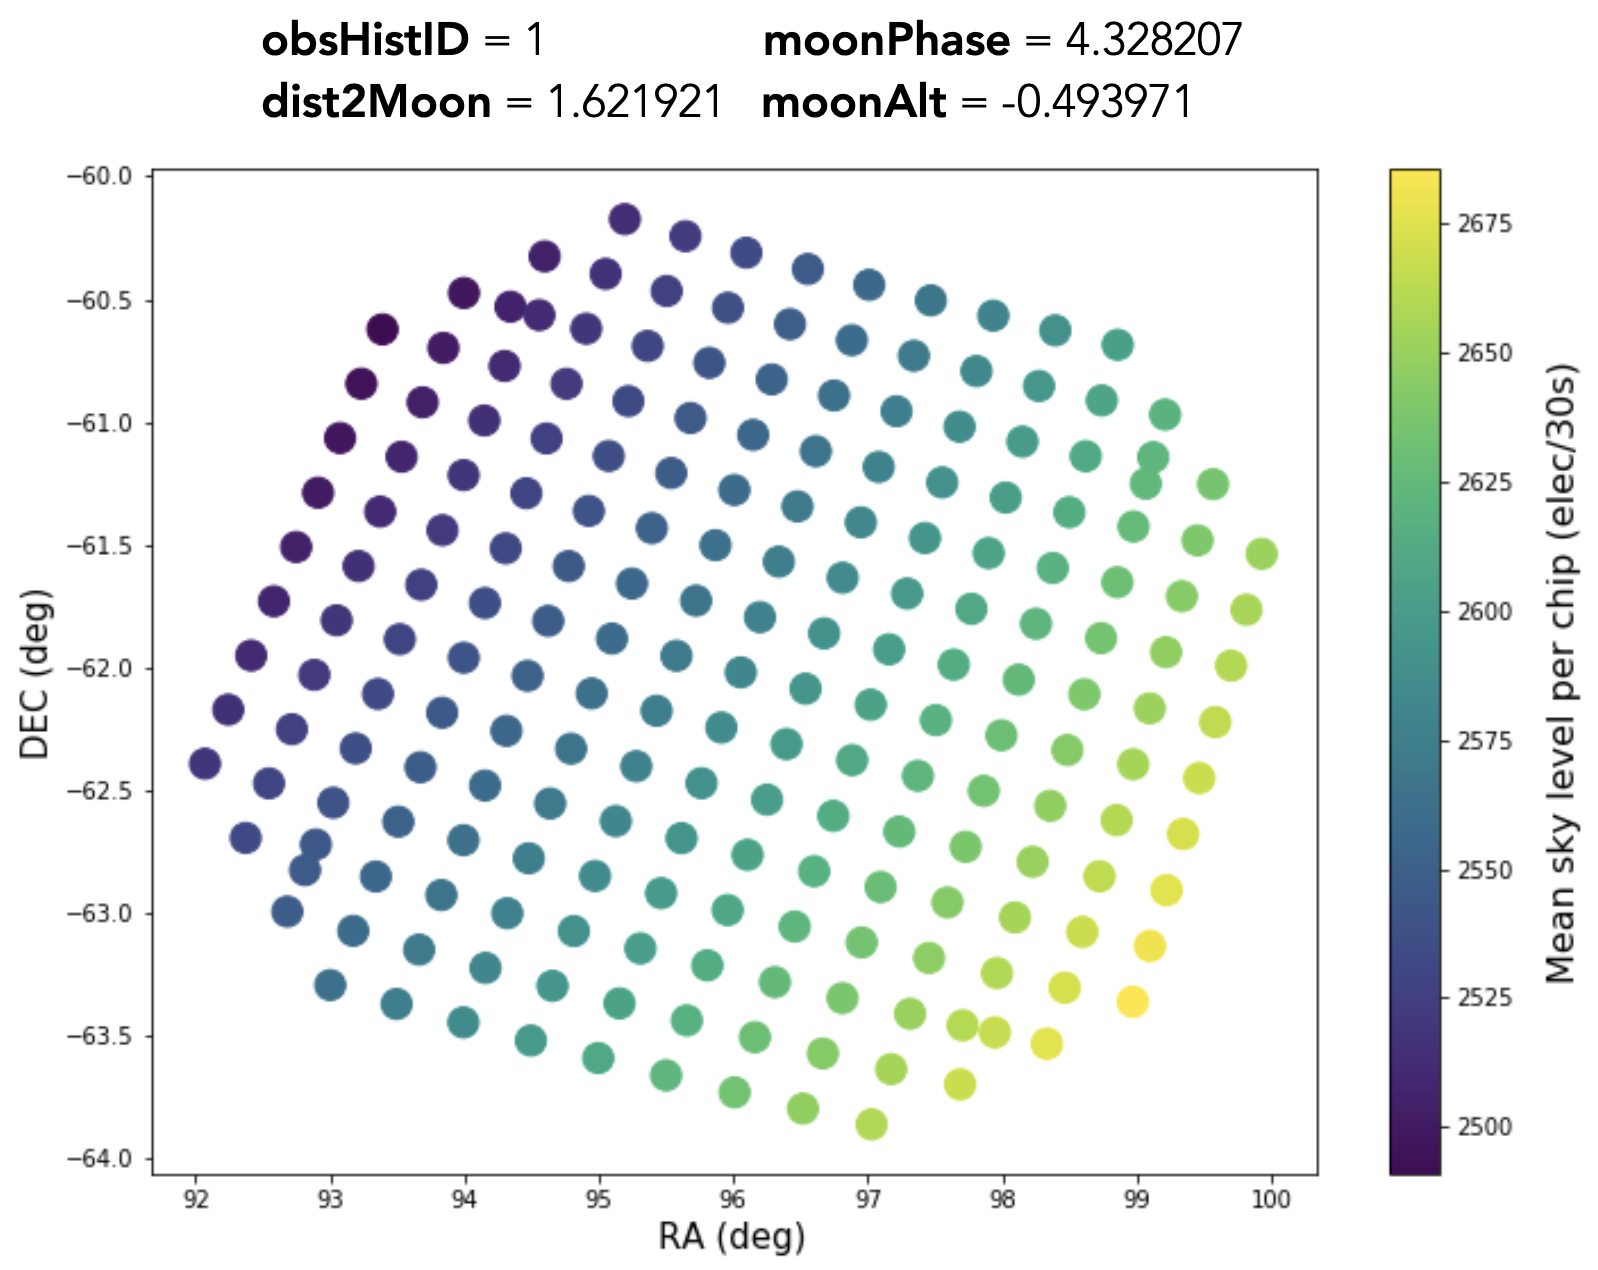
\includegraphics[width=8cm]{images/sensors/skymodel1.jpg}
\caption{No noise.}
\label{fig:skymodel1}
\end{figure}

The results in the r-band are shown in Fig. \ref{fig:skymodel1} for relatively good observing conditions where there is very little contamination from the moon. Each point in the plot represents an individual sensor on the LSST focal plane. The color corresponds to the mean sky level per chip in electrons per exposure. Because sky noise is Poisson distributed, the scale for variations across the focal plane is given by the square root of the number of counts at its center. This scale was used to compare the implementation of a per chip sky model versus a model that uses a single sky level for the entire focal plane. 

\begin{figure}
\centering
\begin{subfigure}[b]{.32\textwidth}
  \centering
  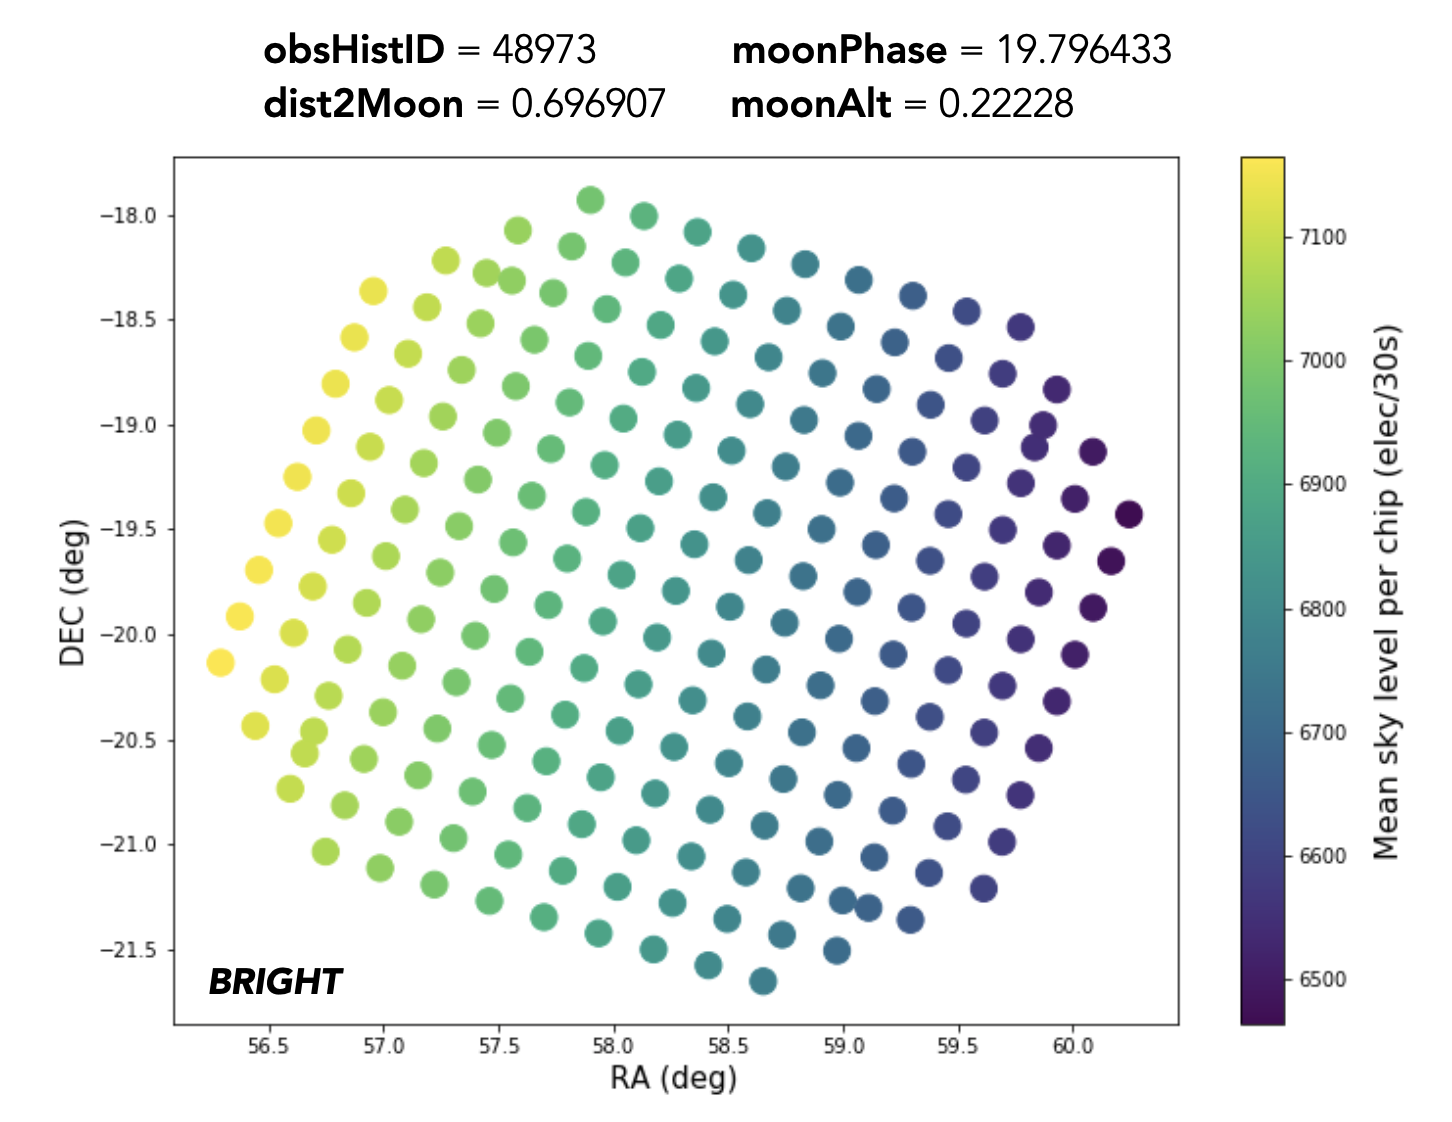
\includegraphics[width=\textwidth]{images/sensors/skymodel_dark.jpg}
  \caption{Dark.}
  \label{fig:sub1}
\end{subfigure}%
\begin{subfigure}[b]{.32\textwidth}
  \centering
  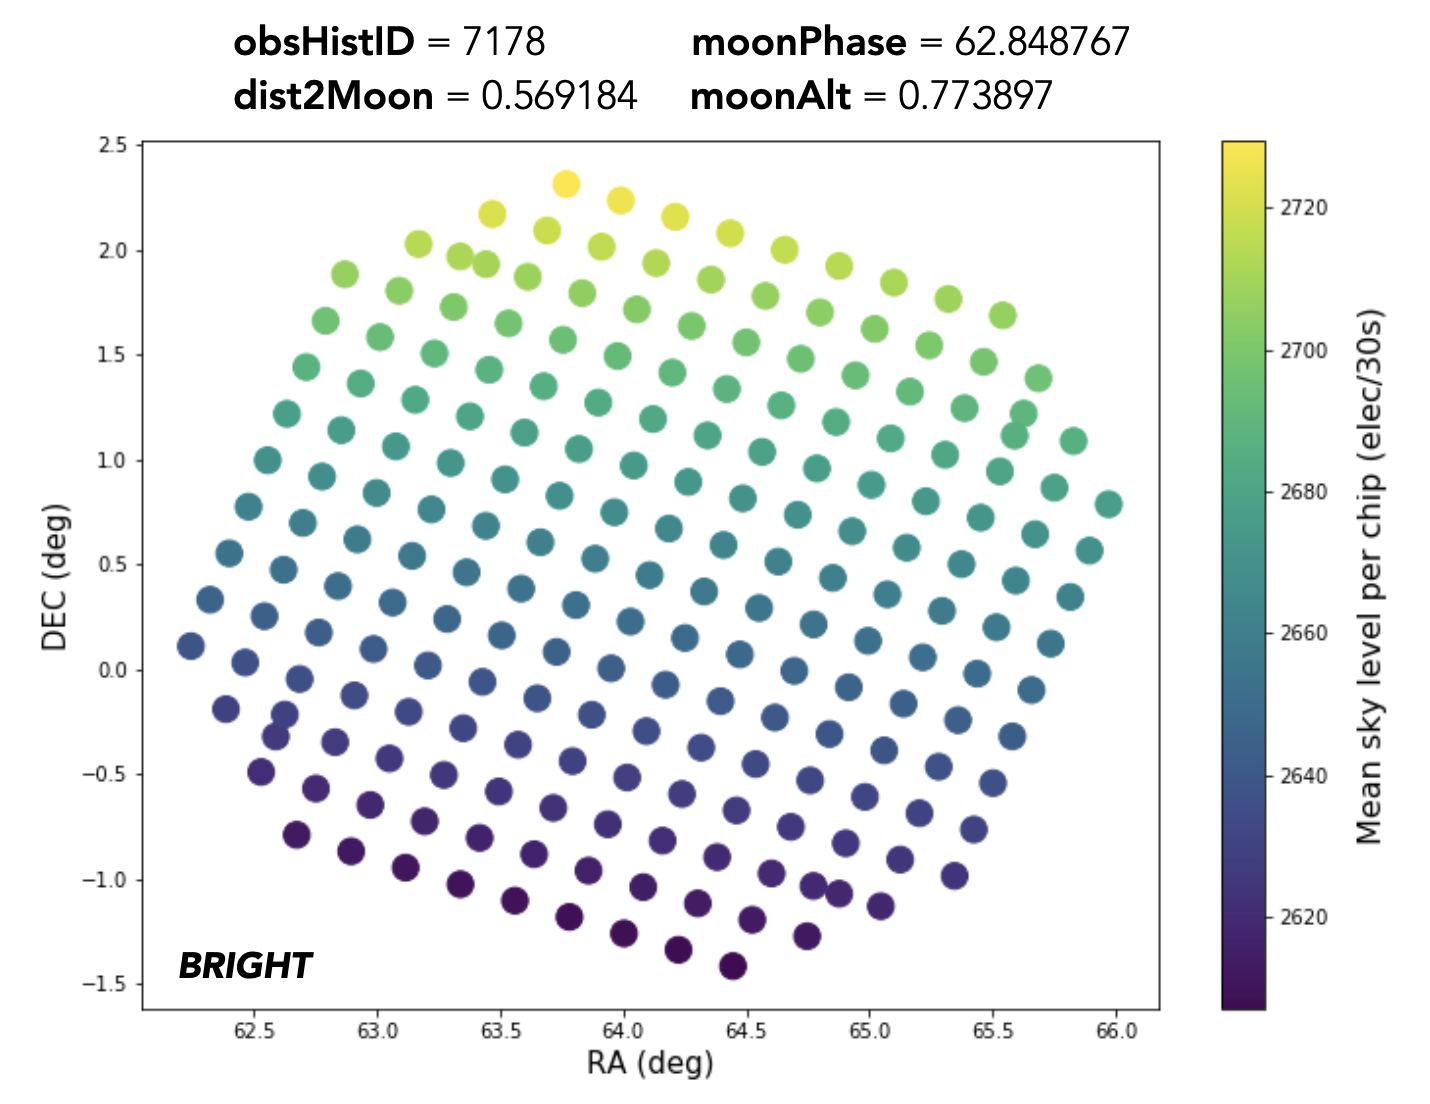
\includegraphics[width=\textwidth]{images/sensors/skymodel_bright1.jpg}
  \caption{Bright.}
  \label{fig:sub2}
\end{subfigure}
\begin{subfigure}[b]{.32\textwidth}
  \centering
  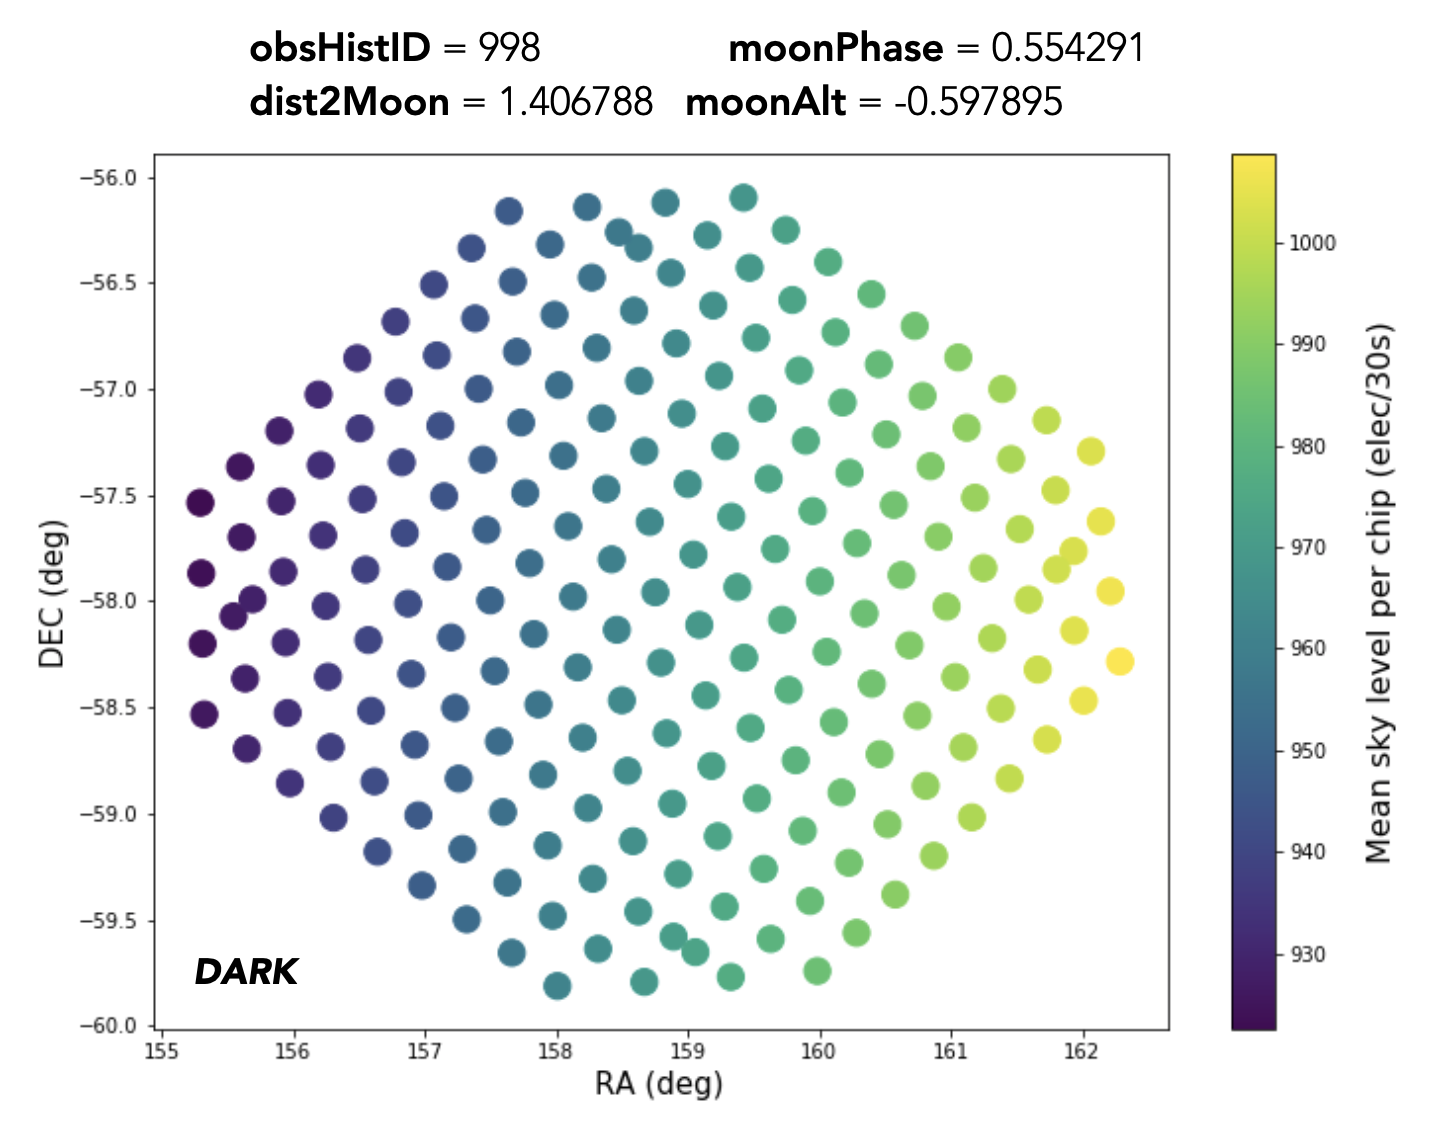
\includegraphics[width=\textwidth]{images/sensors/skymodel_bright2.jpg}
  \caption{Bright.}
  \label{fig:sub2}
\end{subfigure}
\caption{moonPhase (0=new, 100=full), dist2Moon (rad), moonAlt (rad).}
\label{fig:skymodel2}
\end{figure}

In this case, the per chip variation is around 175 sky counts, which is significant compared to the spread around the number of counts at the focal plane center, which is approximately $\sqrt{2600} = 50$. This is based on the uncertainty on the mean number of counts in a single exposure, given by $\sqrt{N}$, where N is the number of counts at the center of the focal plane. Fig. \ref{fig:skymodel2} shows three more examples in both bright and dark conditions. Once again, in all three cases it is clear that the range in sky counts across the focal plane per chip is dominant over the scale for variations based on the number of counts at the center.

\begin{figure}
\centering
\begin{subfigure}[b]{.5\textwidth}
  \centering
  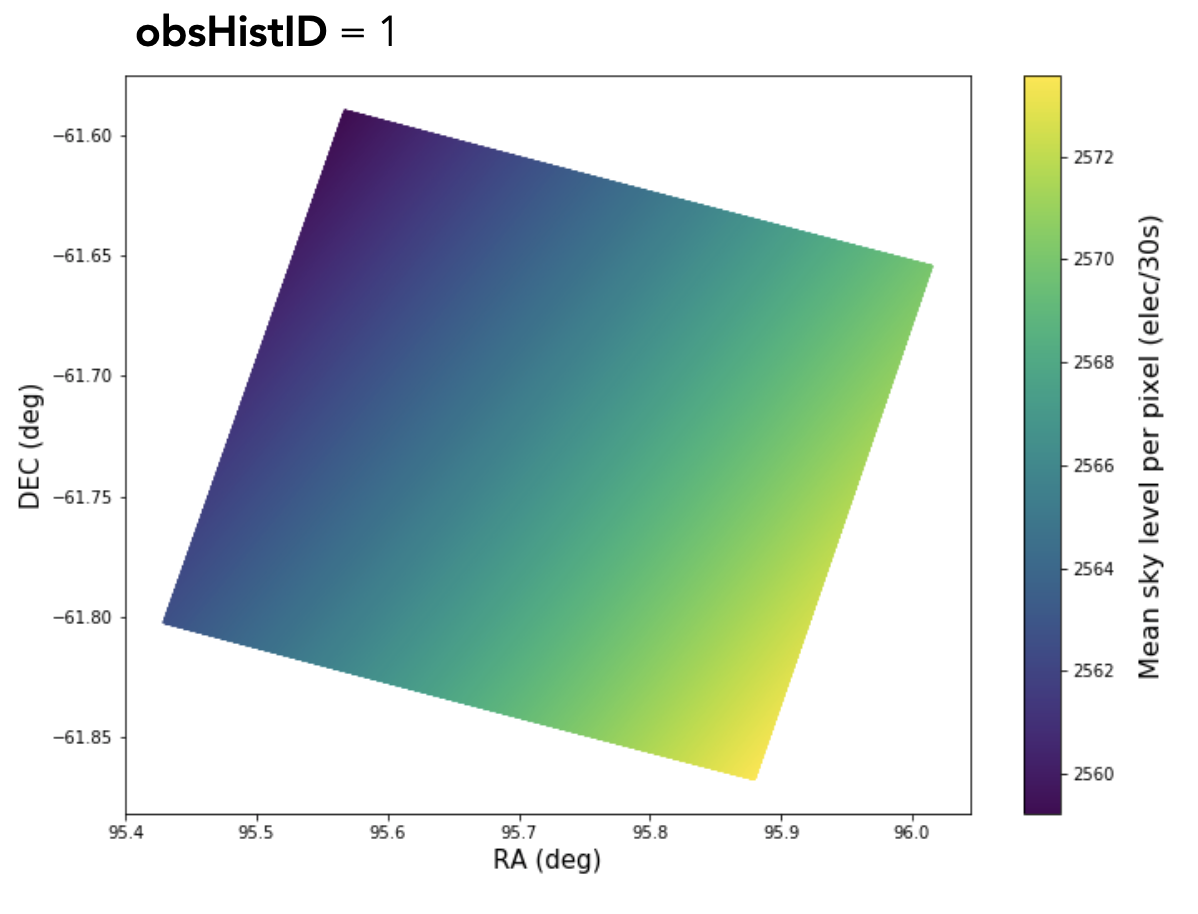
\includegraphics[width=\textwidth]{images/sensors/perpixel1.jpg}
  \caption{obsid1}
  \label{fig:sub1}
\end{subfigure}%
\begin{subfigure}[b]{.5\textwidth}
  \centering
  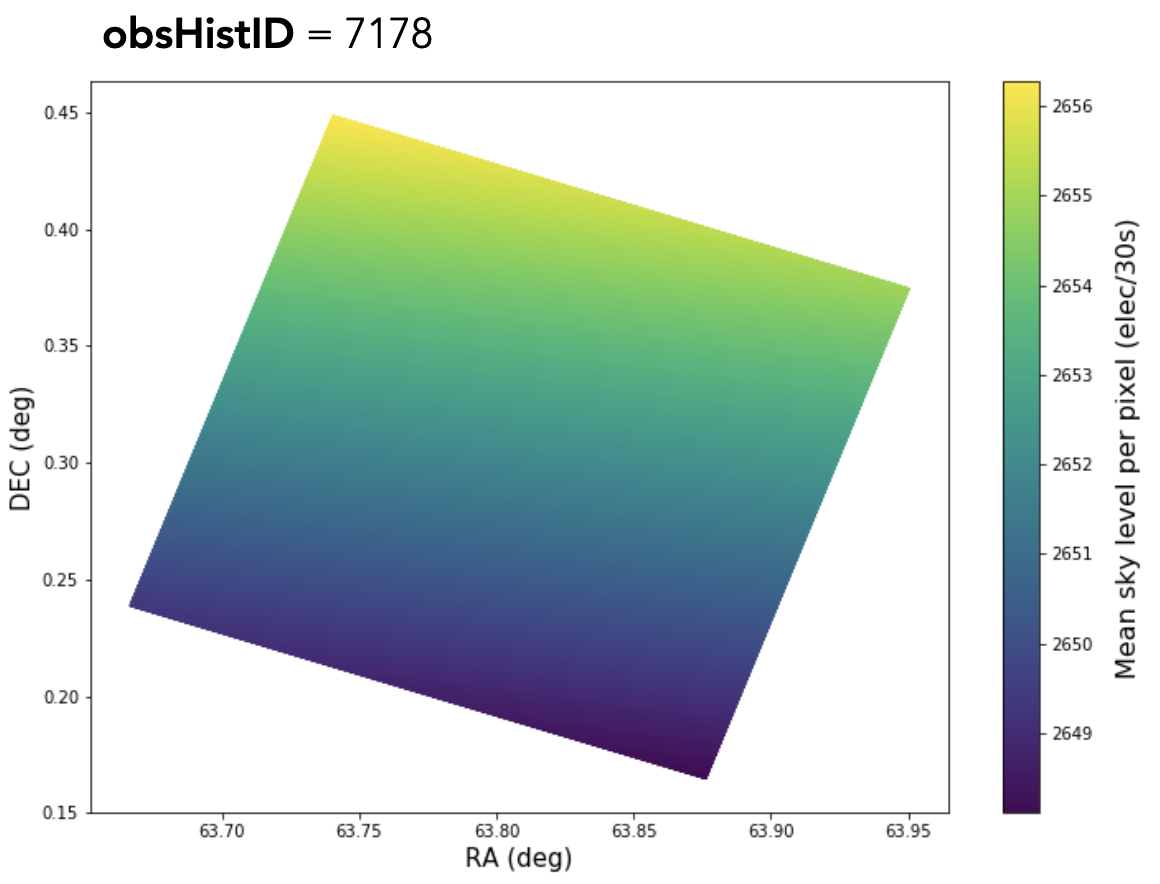
\includegraphics[width=\textwidth]{images/sensors/perpixel2.jpg}
  \caption{obsid7178}
  \label{fig:sub2}
\end{subfigure}
\caption{Per-pixel variation is sub-dominant.}
\label{fig:skymodel3}
\end{figure}

A natural follow-up was to investigate whether it was necessary to add the sky level per-pixel as opposed to per chip. Fig. \ref{fig:skymodel3} shows the per-pixel sky counts in the r-band for two different observations. It's clear that the per-pixel variation is sub-dominant and that accounting for the sky level based on the center of each pixel is sufficient. 

\section{Simulating the brighter-fatter effect}

\subsection{The brighter-fatter effect}

The LSST will generate shear and mass maps over a redshift range of $0.3<z<3.0$ (?) using weak gravitational lensing. The lensing sample will include an unprecedented number of galaxies to the point where statistical errors will be reduced and systematic errors will dominate. Thus in the era of precision astronomy, managing the error budget means accounting for systematic effects that were previously sub-dominant. This includes, for example, errors in the estimation of redshift and cosmic shear. 

One of these errors is the PSF shear systematic error. The PSF, or point spread function, is the two-dimensional flux representation of a point source on the focal plane. Contributions to the PSF come from atmospheric turbulence (or seeing) as well as the instrument, which includes telescope optics, deviations from a flat focal plane and sensor anomalies. Together these effects manipulate point sources such that they are rendered as anisotropic blobs on the detector. 

On the level of the sensors, there is a flux-dependence of the PSF due to the electrostatic (Coulomb) repulsion of charges as they near the collecting wells, or pixels. This phenomenon, where accumulated charge in a pixel repels incoming charges into adjacent pixels, is called the brighter-fatter effect. The net result is a mismatching of photo-electrons to pixels, which effectively distorts the dimensions of a pixel from its original square boundaries.

The brighter-fatter effect has the greatest impact on galaxies used for weak lensing, where measurements are dominated by faint galaxies. It may seem contradictory that it would be a greater issue for low-flux galaxies, since its effect is noticeable and increases for brighter and brighter sources. However the reason for this is that for a given galaxy, its observed shape is a convolution of its true shape with the PSF; and while the telescope PSF is the same for each exposure, the atmospheric PSF is not only stochastic, but it is derived from images of bright (Milky Way) stars. The impact of brighter-fatter is therefore negligible for faint galaxies whose peak flux is much lower than the background sky level, but extremely consequential for images of bright stars whose sizes and shapes are measured and used to build a fitting function to extract across the PSF across the focal plane (1703.05823). Failing to mitigate the systematic shape error of these stars would make them poor PSF calibrators for the purposes of weak lensing, ultimately resulting in incorrect PSFs for faint galaxies (1710.03235v1). 

\begin{figure}
\centering
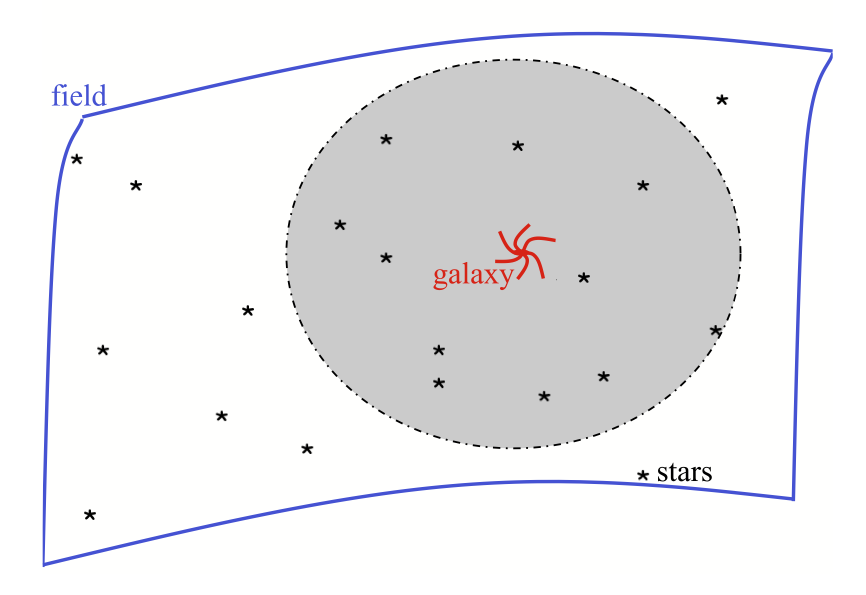
\includegraphics[width=8cm]{images/sensors/psf_interp.jpg}
\caption{Paulin-Henriksson S, Amara A, Voigt L, Refregier A, Bridle SL. 2008. A&A 484:67–77 (via 1710.03235v1).}
\label{fig:skymodel1}
\end{figure}

The cosmological shear signal is typically on the order of 1\% (need source), whereas brighter-fatter alters the sizes of bright stars by 1\% or less (1703.05823), easily masking any shape distortions due to lensing. For Stage-IV experiments, the upper limit on PSF shear systematics is 3 x 10-4 (1506.06427)

From (1703.05823): ``To meet precision WL goals of LSST, it is required to reduce the systematic multiplicative shear bias to the range of 10-3-10-4 and to reduce the additive PSF shear bias to 10-4.'' (What's the difference between multiplicative + additive bias? - Rachel's paper says: additive shear bias is error in PSF shape model, multiplicative shear bias is error in size model)

From (1710.03235v1): ``Since the weak lensing shear is so small compared to the intrinsic, randomly-oriented galaxy ellipticities (often called “shape noise”), averaging over very large ensembles of galaxies is the key to achieving small statistical errors. Indeed, this shape noise dominates over the impact of pixel noise in galaxy shape estimation for nearly all galaxies above detection significance of ∼5. Hence weak lensing measurements generally use galaxies that are as faint and small as possible, down to the limit imposed by the need to control systematic uncertainties.''

From (https://arxiv.org/pdf/astro-ph/0003014.pdf): ``Theoretical expectations for this “cosmic shear” on 10-30 arcminute angular scales range from a few percent for standard cold dark matter to less than one percent for an open universe which would expand forever.8–15 The typical background galaxy has an intrinsic ellipticity of roughly 30\%, so that many thousands of source galaxies must be averaged together to detect the small change induced by cosmic shear.''

Circle back at some point to why they are anisotropic (because of the channel stops).

\subsection{Characterizing brighter-fatter with PoissonCCD}

(Explain work being done to characterize and remove it: solve Poisson equation on a 3D lattice (1911.09567))

(From Craig's PoissonCCD paper (1911.09038))

- CCD simulator, sets parameters via a config file (state what can be controlled here, ie number of electrons, back bias/voltages, z/height, etc)
- Numerically solves Poisson's equations within a simulation volume consisting of silicon bulk, with boundary conditions are determined by the potentials applied to the bulk surface. The CCD solver then calculates the potentials and electric fields inside the silicon. It then propagates electrons from the top of the CCD (does it matter what wavelength they have/where in the bulk they are generated? or is it all in a single band/wavelength?) Effects of brighter-fatter are discerned by pixel boundary distortions caused by charge belonging to one pixel ending up in adjacent pixels. 
- The process goes like this: give 1 pixel a fixed amount of charge (this is at the bottom already, not the top?) and give all the rest zero, then calculate all the electric fields/potentials, the propagate electrons through the bulk, then do a binary search to find bifurcation points that determine the pixel boundaries, then plot distortion in pixel boundaries/area due to accumulated central pixel charge
- The result is that the central pixel loses area while the surrounding pixels gain area (in an asymmetric fashion, with more area in pixels in y-direction - is this because this is parallel to the buried channel stops?)



%%% Local Variables: ***
%%% mode: latex ***
%%% TeX-master: "thesis.tex" ***
%%% End: ***
